\begin{figure*}[ht]
    \centering
    \begin{minipage}{0.45\textwidth}
        \centering
        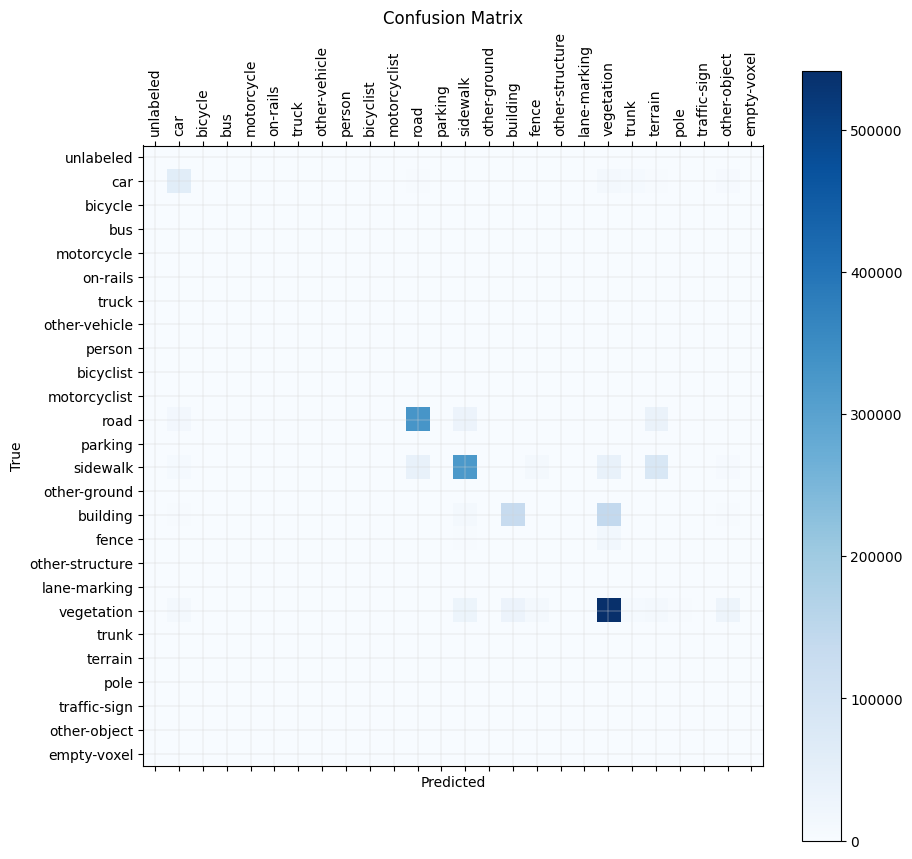
\includegraphics[width=\textwidth]{images/confusion_matrix.png}
        \caption{Confusion matrix}
        \label{fig:matrix}
    \end{minipage}\hfill
    \begin{minipage}{0.45\textwidth}
        \centering
        \begin{tabular}{r|c|c|c|l}
            \multicolumn{5}{c}{\rule[-0.4cm]{0pt}{1.2cm}}  \\
            \multicolumn{1}{c}{} & \multicolumn{3}{c}{\rule[-0.4cm]{0pt}{1cm} VUE-net} & \multicolumn{1}{c}{} \\ \cline{2-2} \cline{4-4}
            $mAccuracy$  & \rule[-0.4cm]{0pt}{1cm} $0.692$ & & $2.197s$ & $Vox.\;time$   \\ \cline{2-2} \cline{4-4}
            $mPrecision$ & \rule[-0.4cm]{0pt}{1cm} $0.427$ & & $0.011s$ & $Pred.\;time$  \\ \cline{2-2} \cline{4-4}
            $mRecall$    & \rule[-0.4cm]{0pt}{1cm} $0.327$ & & $0.911s$ & $Back.\;time$  \\ \cline{2-2} \cline{4-4}
            $F1-score$   & \rule[-0.4cm]{0pt}{1cm} $0.371$ & & $3.119s$ & $Tot.\;time$ \\ \cline{2-2} \cline{4-4}
            \multicolumn{5}{c}{\rule[-0.4cm]{0pt}{1.2cm}}  \\
        \end{tabular}
        \captionof{table}{Model performance}
        \label{tab:metrics}
    \end{minipage}
\end{figure*}

\begin{figure*}[ht]
    \centering
    \begin{subfigure}[b]{0.45\textwidth}
        \centering
        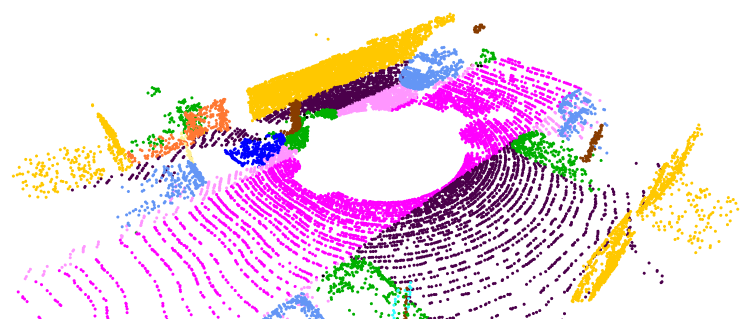
\includegraphics[width=\textwidth]{images/true.png}
        \caption{True labels}
        \label{fig:true}
    \end{subfigure}
    \hfill
    \begin{subfigure}[b]{0.45\textwidth}
        \centering
        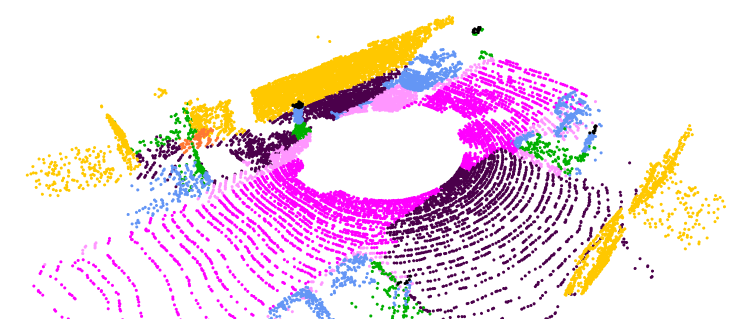
\includegraphics[width=\textwidth]{images/pred.png}
        \caption{Predicted labels}
        \label{fig:pred}
    \end{subfigure}
    \caption{True and predicted labels for pointcloud 55}
    \label{fig:visual}
\end{figure*}

The dataset made of 1000 sample was split into subsets of 750, 150 and 100 samples that correspond respectivly
to training, validation and test sets. In addition, samples from the training set were shuffled before being used.
The training phase was set such that for a determined number of epochs, the samples from the proper
set were loaded in batches of 10, rotated by 90 degrees around the z-axis by a random number
of times in the range 0-3 (to embedd robustness to such rotations) and then given as 
input to the model, which performed the forward and backward propagation processes.
For this last operation, a loss function is needed.
We initially opted for the CrossEntropy loss, but we soon encountered poor results. This was due to the class imbalance of the
samples towards the "empty voxel" class. This happened for two reasons: first, by using voxelgrids instead of pointclouds
we introduced lots of empty space in our samples that had to be encoded too; second, the sampling of the pointclouds may lead 
to creating empty voxels that actually contain points.
We tried to address this issue by using the weighted version of CrossEntropy loss.
The weights were computed as as the inverse of the normalized sum of the class membership distribution probabilities 
over all voxels in the training set samples.
Even if this approach showed better performance, the class imbalance was too severe and the obtained results were not acceptable.
This lead us to our final choice for the loss function, Dice Loss.
This function allowed for fairly good model performance after training. This result is caused by the fact that Dice Loss considers 
the intersection over the union (IoU) of the predicted and true positive regions, which makes it particularly sensible to small 
and underrepresented classes.
After each epoch, validation was performed through the ensemble version of the model
to assess the current model performance and save it only if it was the best one seen so far. 
As for the Validation Loss we decided to use "one minus" the accuracy metric computed on the validation set samples.
This value is computed by a function that confronts each true and computed label tensors in their one-hot encoded version 
(argmax set to 1, others to 0) and returns the normalized count of pairs of different tensors.
By training our network for 50 epochs while relying on Adam optimizer with learning rate 0.001, we achieved a validation loss value of 0.280, which
means that the model correcly labels 72.0\% of the samples voxels in the validation set.